\chapter{Ray tracing}
\label{chap:RT}
As mentioned in the previous chapter, we want to simulate the signal a neutrino event
would produce in the detector. The neutrino event generates radiowaves that end
up at our detector, but as the ice has a continuously varying density, these radiowave
paths need to be computed.

In this chapter we'll go more in-depth as to how the radio wave paths get
simulated in ice within the NuRadioMC framework.
\section{Wave propagation}
\label{sec:WaveProp}
\begin{figure}[h!]
	\centering
	\includegraphics[width=0.7\textwidth]{DirectNReflected.pdf}
	\label{fig:PathIllu}
	\caption{Simulated radio wave paths from a source to a detector, these always come in a pair 
	if it's an in-ice source due to the density gradient of the ice and the reflective ice-air boundary.}
\end{figure}
There is a multitude of photons coming from our event but only the ones
in line with the cherenkov cone are strong enough to be detectable.
We thus only need to concern ourselves with simulating those.

The way we simulate the strongest waves propagating to the detector from a
radio source is through a process called ray tracing which we'll explain shortly, 
an illustration of the final result of ray tracing is shown in figure \ref{fig:PathIllu}.  

The amount of solutions (i.e how many radio wave paths exist between our source and the detector)
and how the waves are bent are consequences of the
properties of the ice we work in.  In a dielectric medium a ray propagates with
its signal wave-speed determined by the local index of refraction as $v =
c/n$. But the effect on speed isn't the only property the index of refraction has
which we'll need to concern ourselves with, another one is the breaking of the path,
but to understand that effect in continuous media we'll first need to talk about Snell's law. 

If a ray propagates towards a boundary dividing 2 media with different indexes
of refraction, the ray will refract and the refracted angle can be found from
Snell's law:
\begin{equation}
	n_i\sin{\theta_i} = n_o\sin{\theta_o}
\end{equation}
Where n is the index of refraction, $\theta$ the angle with respect to the
surface normal and "i" and "o" indicating incoming and outgoing respectively.
The system we'll consider however, isn't homogeneous with some specified
boundary. Ice in Greenland has a continuously varying density and
index of refraction.

How do we know how the waves propagate in such a medium?  The software we'll be
using to simulate how the radio waves behave is called \textit{Radiopropa}
\cite{Winchen_2019}. As simulations of the wave propagation in full detail with
the finite-differences-time-domain (FDTD) technique \cite{1138693} (solving
maxwells equations on a grid) are, even though they are more accurate, quite time
consuming. The authors of radiopropa opted to build their program on
geometrical optics, i.e ray tracing. A path of a ray $\mathbf{r}(s)$ with path
parameter s in a medium with index of refraction n($\mathbf{r}$) is described
by the eikonal equation\cite{herman2019treatise}:
\begin{equation}
	\frac{d}{ds}\left(n(\mathbf{r})\frac{d\mathbf{r}}{ds}\right) = \mathbf{\nabla} n
\end{equation}
In radiopropa the local paraxial approximation (small angle approximation) is
used, i.e if we assume that in any individual step of the algorithm the change
of the refractive index along the path $ds$ is small it's possible to rewrite
the equation as:
\begin{equation}
	n(\mathbf{r})\frac{d^2\mathbf{r}}{ds^2} \approx \mathbf{\nabla} n
	\label{eqn:radiopropaformula}
\end{equation}
Which is then numerically solved using the Cash–Karp method.  The way you would
go about using this program is thus: given a starting point (e.g a supposed
neutrino interaction point), "shoot" your ray in a
certain direction. Radiopropa will then compute the path the ray takes. 
If you chose your direction right, this ray will at some point cross an
"end point" you gave it (e.g the location of the detector) at which point it will
stop simulating. Meaning that you now have computed the path from a start point in ice
to an end point.

The difficulty in this matter is choosing the direction right so the ray
crosses paths with the end point, for this a wrapper algorithm is needed which we'll
get to later.  If there are boundaries (such as in-ice defects or the ice-air surface) these
are treated separately within radiopropa using Snell's law. 
\section{Ice model}
\label{section:Ice Model}
Radiopropa, as previously described, is based on solving equation \ref{eqn:radiopropaformula}.
This equation is dependent on the local index of refraction $n(\mathbf{r})$ for which
we'll thus need a model. But before we can derive a model we'll need to talk about the
density-depth relation.

Due to the way the ice bonds there will be more air trapped in between the
molecules closer to the surface than at greater depths where the pressure due
to the overhead ice prevents this.  Due to this air being trapped, the density
of ice will be smaller closer to the surface than at greater depth.  The region
where this air occurs in the ice is called the firn\cite{Firn} as to
distinguish it from glacial ice which is ice at large depths with nearly no air
trapped.

Purely from classical gravity and density considerations it can be derived that
the density scales exponentially. To see this let's consider a sheet of ice in
the Greenland firn with a surface A at a depth z and with a width dz, the extra
pressure this sheet of ice exerts on the ice just below it is:
\begin{equation}
	d\sigma = \frac{dF}{A} = -\frac{gdM}{A} = -g\frac{A\rho(z)dz}{A} = -g\rho(z)dz
\end{equation}
with $\rho(z)$ the depth-dependent density. The proportional change in air
space is assumed to be proportional to the change in
pressure\cite{herron_langway_1980}:
\begin{equation}
	\frac{dV}{V} \propto d\sigma
\end{equation}
As the volume scales inversely with the density let's assume the relation $V \propto (\rho_i - \rho)$ with
$\rho_i$ the density of pure ice, this yields:
\begin{equation}
	\frac{d\rho}{\rho_i - \rho} \propto \rho dz
\end{equation}
Which can be solved to give
\begin{equation}
	\rho = \frac{A\rho_i e^{z/z_0}}{1 + Ae^{z/z_0}}
\end{equation}
The following function was also empirically fitted:
\begin{equation}
	\label{eqn:myderiexp}
	\rho = \rho_0 e^{z/z_0} + B
\end{equation}
Figure \ref{fig:DensityMeasurements} shows how both of these functions fit the
density-depth data\cite{alley_koci_1988}\cite{hawley_morris_mcconnell_2008}.  
\begin{figure}
  \centering
	\includegraphics[width=0.5\textwidth]{Density_measurements2.pdf}
	\caption{Illustration of the shortcomings of the analytical models}
	\label{fig:DensityMeasurements}
\end{figure}
Now that we have a model for the density-depth curve we can link this to the
index-depth relation we need for radiopropa.  The dependence of the dielectric
constant on density for ice can approximately be given by\cite{Robin}:
\begin{equation} 
	\epsilon(z) \approx (1 + 0.845\rho(z))^2 
\end{equation} 
Here $\rho$ is called the \textit{specific gravity} as to make the equation
dimensionally correct, this is the same as the density in g/cm$^3$ but stripped
off its units.  As the dielectric constant is the square of the index of
refraction we can find an approximate index-density relation:
\begin{equation} 
	n(z) \approx 1 + 0.775\frac{\rho(z)}{\rho_0} \approx 1 + 0.78\frac{\rho(z)}{\rho_0} \label{eqn:Schytt}
\end{equation} 
Where we introduced $\rho_0$, the density for solid ice (917 kg/m³).  
Now that we have a linear relation between the index of refraction and the density
and also a model for the density-depth relation (equation \ref{eqn:myderiexp}) these two can
be combined to form the \textit{single exponential model}
\begin{equation}
	\label{eqn:expn}
	n(z) = n_{ice} - \Delta n e^{z/z_0}
\end{equation}
with $n_{ice}$ the refractive index of solid ice and $\Delta n = n_{ice} - n_s$
with $n_s$ the index of refraction of snow. 

Using this exponential model for radiopropa has a huge advantage as it's
analytically solvable, meaning that we can know which direction we'll have to
shoot our ray in after the location of the neutrino interaction and the
detector are specified. The ray tracing algorithm developed using this
exponential index is called the \textit{analytic ray tracer}.

\section{Shortcomings of the exponential ice model}
As can be seen from figure \ref{fig:DensityMeasurements}, there is a
discrepancy between the single exponential fit used for the exponential model
and the density data, especially between 40 and 120 meters of depth where the
phased array is located.  This discrepancy could imply that the analytic ray tracer will
make slightly wrong predictions.  This is why the development of a different
ray tracer was needed which will be able to handle more complex ice models. One
such ray tracer, called the iterative ray tracer, will be explained in section \ref{sec:Iterative} but this ray
tracer has its shortcomings. That's why we found that the development of a new ray tracer
was needed which is the partial work of this thesis and we'll get to that ray
tracer in chapter \ref{chapter:hybrid}.

\begin{figure}
  \centering
  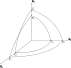
\includegraphics[width=0.5\textwidth]{figures/Fresnel.pdf}
  \caption{The three unit axes each have 2 possible wave speeds. E.g if a wave would
  travel along $\mathbf{e}_1$, depending on the polarization it could travel at a speed $C_3$ or
  at a speed $C_2$. The exponential model assumes all speeds to be the same, i.e $C_1=C_2=C_3=c/n$}
  \label{fig:Fresnel}
\end{figure}

There is also another effect worth mentioning that the exponential model
doesn't account for which might become important in the future: birefringence.
Up until now we have implicitly assumed that ice is isotropic meaning that both
its permittivity $\varepsilon$ and its permeability $\mu$ are scalars but
these could very well be tensorial in nature for radio waves in ice. In
general, after calculating this tensorial nature through you'd find that in
every direction two different indices of refraction can be found implying two
different types of waves each propagating with a different speed as illustrated
in figure \ref{fig:Fresnel}.  Of these two possible speeds in a direction, which the waves actually
follow is then dependent on the polarization of the wave, which in our case thus depends
on the Askaryan effect (see section \ref{sec:Askaryan}).  This optical property
coming from the anisotropic nature of the material is what's called
\textit{birefringence}.  Birefringence has been researched for it's
implementation into the simulation software NuRadioMC\cite{Heyer2023}.
\newpage
\section{Iterative ray tracer}
\label{sec:Iterative}
To work with more complex index-depth relations there's a need for a
new algorithm which is able to find the angle with which radiopropa should
shoot its ray if given the neutrino interaction and detector location.

To this end the iterative ray tracer \cite{2022icrc.confE1027O} was developed.
As can be derived from its name, it iteratively searches the path a ray might
take. We'll now explain the workings of the first part of the algorithm, a handy
accompanying illustration is given in figure \ref{fig:Illustration of iterative algorithm}.
\begin{figure}
  \centering
  \includegraphics[width=0.8\textwidth]{algoillu.pdf}
  \caption{Illustration of the setup. The red cross is the neutrino interaction vertex, the blue dot is the detector,
  the observer sphere around the detector stops the simulation counting it as a solution and the other observers (other lines with eyes) don't count the ray as a solution.}
  \label{fig:Illustration of iterative algorithm}
\end{figure}
\subsection{Setup}
Say we have a neutrino interaction point $\mathbf{X}_i$
(the red cross on the figure) and a detector located at $\mathbf{X}_d$ (the
blue dot on the figure), the algorithm starts by constructing an
\textit{observer} sphere with radius $r_1$ with the detector, located at $\mathbf{X}_d$, as the
center.  This means that any ray that gets shot and propagates to the sphere
will get stopped and counts as a solution.  Then, to reduce the time spent simulating, there are also observers placed
whose purpose is to stop the ray tracing but not count the observed signal as a solution.
One such observer is placed 
just above the ice surface as a ray that escapes the ice won't be able to make it back, and one
is placed just behind the detector looking from the point of the interaction vertex $\mathbf{X}_i$ as
a ray is not able to reach the detector anymore after it has passed it in the
lateral direction. 

Finally, it's noted that due to the way the ice's index of refraction
continuously increases with depth, rays can't propagate upwards, this means that we only 
have to look for solutions within the angle $\Omega$ which is just the zenith angle the detector
makes with the bottom of the observer sphere.

\subsection{Narrowing algorithm}
Now that the setup has been established we'll just iteratively shoot rays from the neutrino
interaction point starting at an angle $\Delta \theta_1$ then at an angle
$2\Delta \theta_1$, $3\Delta \theta_1$,... Until we have reached $\Omega$. This
process is illustrated on the left side of figure \ref{fig:IterativeWorkings}.
\begin{figure}
  \centering
  \includegraphics[width=0.9\textwidth]{IterativeWorkings.png}
  \caption{Illustration of the steps in the iterative ray tracer, first rays get shot in steps of 0.5°, the ones that end up at the sphere with a 25m radius are colored in green and within these angles the algorithm repeats (middle figure) but now with a smaller
  step and sphere size. \citeFig{2022icrc.confE1027O} }
  \label{fig:IterativeWorkings}
\end{figure}
After we have gone over all the different launch angles we'll have some
solutions (marked in green) and some that don't end up on the sphere around the detector (marked
in red) we can now make the observer sphere's radius smaller ($r_2 < r_1$) and
the step size of the angle smaller ($\Delta \theta_2 < \Delta \theta_1$).  And
again iteratively find the rays which end up on the sphere, only this time
looking within the angles of the solutions of the previous step. We can keep on
making the sphere and step size smaller in iterative steps until we've reached
the precision we want. We then take, for each bunch of solutions within an
angle interval, the most normal to the detector as the final solutions.



